\documentclass[1p]{elsarticle_modified}
%\bibliographystyle{elsarticle-num}

%\usepackage[colorlinks]{hyperref}
%\usepackage{abbrmath_seonhwa} %\Abb, \Ascr, \Acal ,\Abf, \Afrak
\usepackage{amsfonts}
\usepackage{amssymb}
\usepackage{amsmath}
\usepackage{amsthm}
\usepackage{scalefnt}
\usepackage{amsbsy}
\usepackage{kotex}
\usepackage{caption}
\usepackage{subfig}
\usepackage{color}
\usepackage{graphicx}
\usepackage{xcolor} %% white, black, red, green, blue, cyan, magenta, yellow
\usepackage{float}
\usepackage{setspace}
\usepackage{hyperref}

\usepackage{tikz}
\usetikzlibrary{arrows}

\usepackage{multirow}
\usepackage{array} % fixed length table
\usepackage{hhline}

%%%%%%%%%%%%%%%%%%%%%
\makeatletter
\renewcommand*\env@matrix[1][\arraystretch]{%
	\edef\arraystretch{#1}%
	\hskip -\arraycolsep
	\let\@ifnextchar\new@ifnextchar
	\array{*\c@MaxMatrixCols c}}
\makeatother %https://tex.stackexchange.com/questions/14071/how-can-i-increase-the-line-spacing-in-a-matrix
%%%%%%%%%%%%%%%

\usepackage[normalem]{ulem}

\newcommand{\msout}[1]{\ifmmode\text{\sout{\ensuremath{#1}}}\else\sout{#1}\fi}
%SOURCE: \msout is \stkout macro in https://tex.stackexchange.com/questions/20609/strikeout-in-math-mode

\newcommand{\cancel}[1]{
	\ifmmode
	{\color{red}\msout{#1}}
	\else
	{\color{red}\sout{#1}}
	\fi
}

\newcommand{\add}[1]{
	{\color{blue}\uwave{#1}}
}

\newcommand{\replace}[2]{
	\ifmmode
	{\color{red}\msout{#1}}{\color{blue}\uwave{#2}}
	\else
	{\color{red}\sout{#1}}{\color{blue}\uwave{#2}}
	\fi
}

\newcommand{\Sol}{\mathcal{S}} %segment
\newcommand{\D}{D} %diagram
\newcommand{\A}{\mathcal{A}} %arc


%%%%%%%%%%%%%%%%%%%%%%%%%%%%%5 test

\def\sl{\operatorname{\textup{SL}}(2,\Cbb)}
\def\psl{\operatorname{\textup{PSL}}(2,\Cbb)}
\def\quan{\mkern 1mu \triangleright \mkern 1mu}

\theoremstyle{definition}
\newtheorem{thm}{Theorem}[section]
\newtheorem{prop}[thm]{Proposition}
\newtheorem{lem}[thm]{Lemma}
\newtheorem{ques}[thm]{Question}
\newtheorem{cor}[thm]{Corollary}
\newtheorem{defn}[thm]{Definition}
\newtheorem{exam}[thm]{Example}
\newtheorem{rmk}[thm]{Remark}
\newtheorem{alg}[thm]{Algorithm}

\newcommand{\I}{\sqrt{-1}}
\begin{document}

%\begin{frontmatter}
%
%\title{Boundary parabolic representations of knots up to 8 crossings}
%
%%% Group authors per affiliation:
%\author{Yunhi Cho} 
%\address{Department of Mathematics, University of Seoul, Seoul, Korea}
%\ead{yhcho@uos.ac.kr}
%
%
%\author{Seonhwa Kim} %\fnref{s_kim}}
%\address{Center for Geometry and Physics, Institute for Basic Science, Pohang, 37673, Korea}
%\ead{ryeona17@ibs.re.kr}
%
%\author{Hyuk Kim}
%\address{Department of Mathematical Sciences, Seoul National University, Seoul 08826, Korea}
%\ead{hyukkim@snu.ac.kr}
%
%\author{Seokbeom Yoon}
%\address{Department of Mathematical Sciences, Seoul National University, Seoul, 08826,  Korea}
%\ead{sbyoon15@snu.ac.kr}
%
%\begin{abstract}
%We find all boundary parabolic representation of knots up to 8 crossings.
%
%\end{abstract}
%\begin{keyword}
%    \MSC[2010] 57M25 
%\end{keyword}
%
%\end{frontmatter}

%\linenumbers
%\tableofcontents
%
\newcommand\colored[1]{\textcolor{white}{\rule[-0.35ex]{0.8em}{1.4ex}}\kern-0.8em\color{red} #1}%
%\newcommand\colored[1]{\textcolor{white}{ #1}\kern-2.17ex	\textcolor{white}{ #1}\kern-1.81ex	\textcolor{white}{ #1}\kern-2.15ex\color{red}#1	}

{\Large $\underline{12a_{0447}~(K12a_{0447})}$}

\setlength{\tabcolsep}{10pt}
\renewcommand{\arraystretch}{1.6}
\vspace{1cm}\begin{tabular}{m{100pt}>{\centering\arraybackslash}m{274pt}}
\multirow{5}{120pt}{
	\centering
	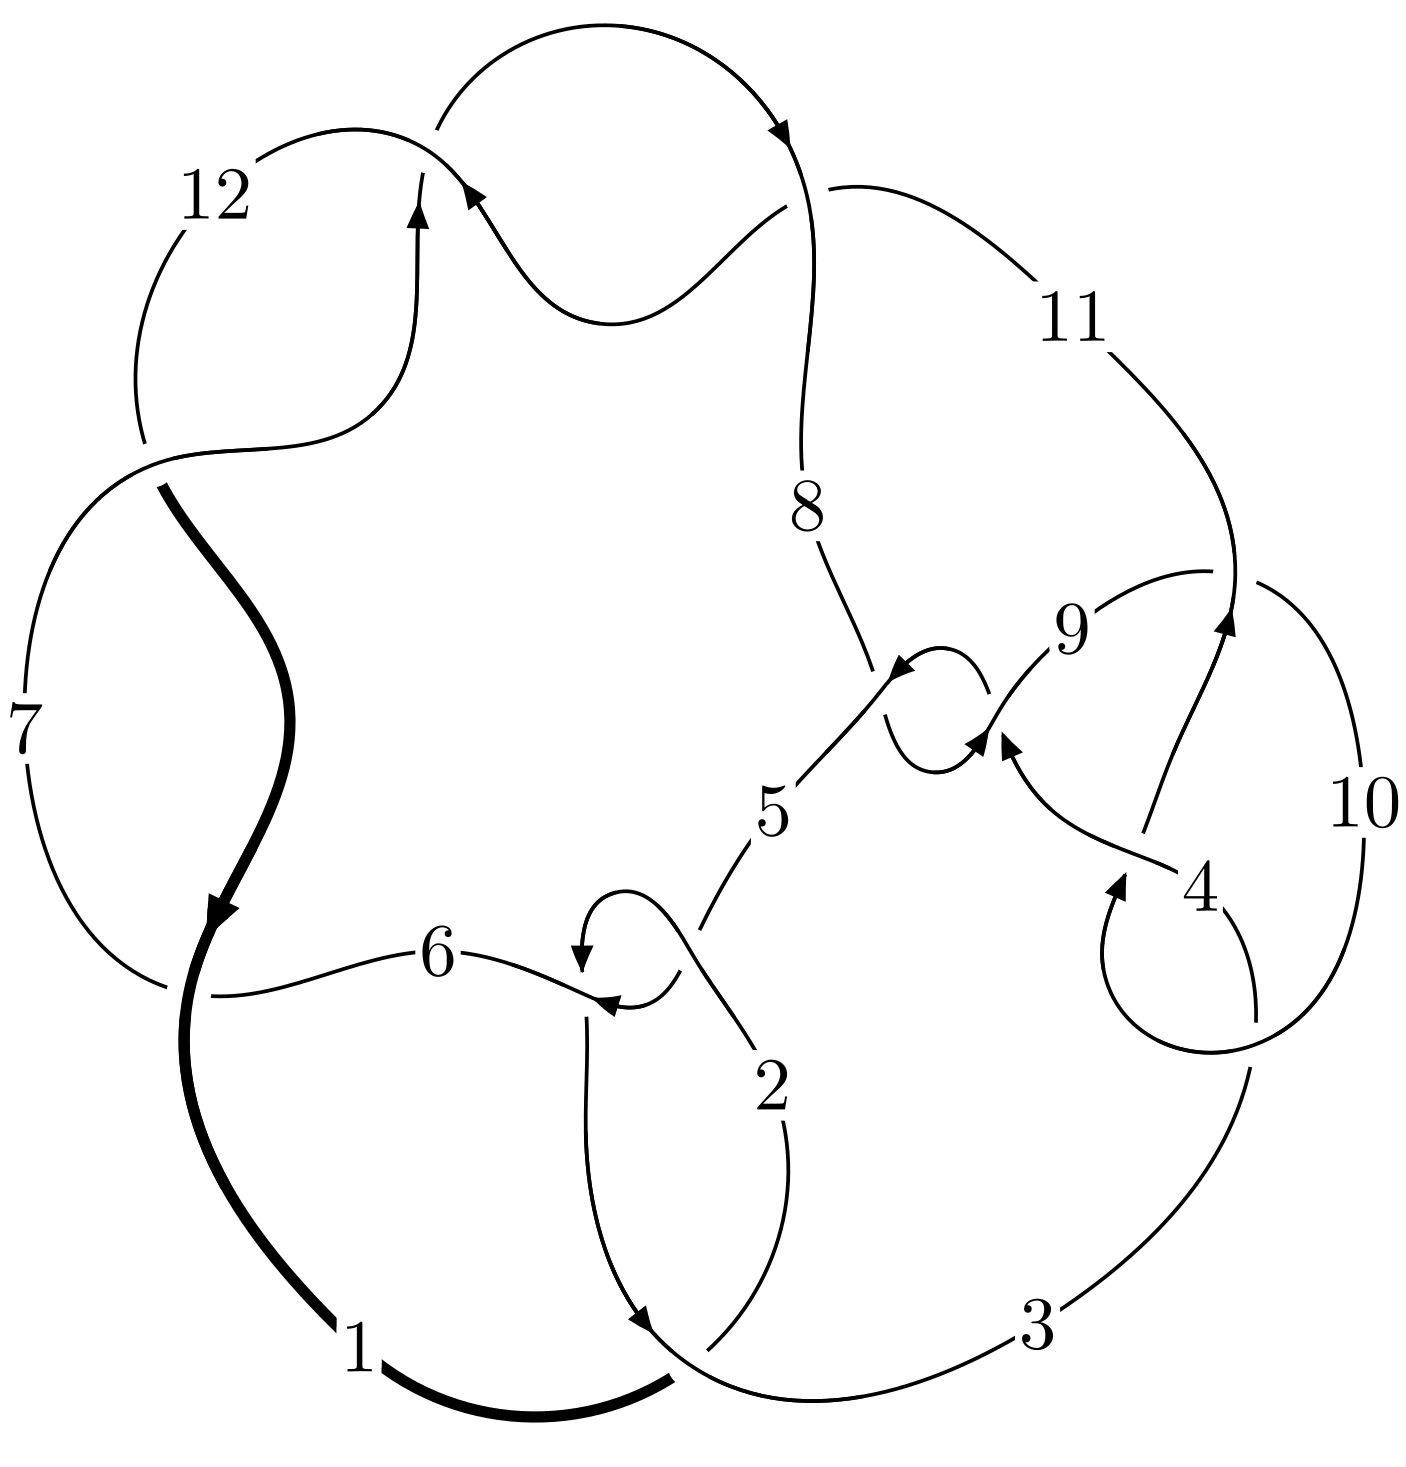
\includegraphics[width=112pt]{../../../GIT/diagram.site/Diagrams/png/1248_12a_0447.png}\\
\ \ \ A knot diagram\footnotemark}&
\allowdisplaybreaks
\textbf{Linearized knot diagam} \\
\cline{2-2}
 &
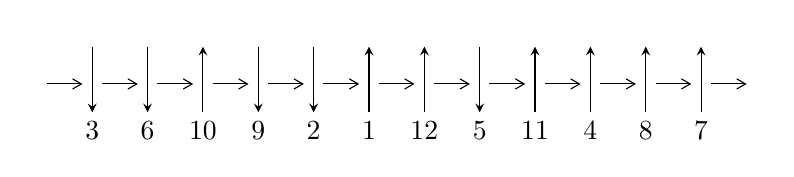
\begin{tikzpicture}[x=20pt, y=17pt]
	% nodes
	\node (C0) at (0, 0) {};
	\node (C1) at (1, 0) {};
	\node (C1U) at (1, +1) {};
	\node (C1D) at (1, -1) {3};

	\node (C2) at (2, 0) {};
	\node (C2U) at (2, +1) {};
	\node (C2D) at (2, -1) {6};

	\node (C3) at (3, 0) {};
	\node (C3U) at (3, +1) {};
	\node (C3D) at (3, -1) {10};

	\node (C4) at (4, 0) {};
	\node (C4U) at (4, +1) {};
	\node (C4D) at (4, -1) {9};

	\node (C5) at (5, 0) {};
	\node (C5U) at (5, +1) {};
	\node (C5D) at (5, -1) {2};

	\node (C6) at (6, 0) {};
	\node (C6U) at (6, +1) {};
	\node (C6D) at (6, -1) {1};

	\node (C7) at (7, 0) {};
	\node (C7U) at (7, +1) {};
	\node (C7D) at (7, -1) {12};

	\node (C8) at (8, 0) {};
	\node (C8U) at (8, +1) {};
	\node (C8D) at (8, -1) {5};

	\node (C9) at (9, 0) {};
	\node (C9U) at (9, +1) {};
	\node (C9D) at (9, -1) {11};

	\node (C10) at (10, 0) {};
	\node (C10U) at (10, +1) {};
	\node (C10D) at (10, -1) {4};

	\node (C11) at (11, 0) {};
	\node (C11U) at (11, +1) {};
	\node (C11D) at (11, -1) {8};

	\node (C12) at (12, 0) {};
	\node (C12U) at (12, +1) {};
	\node (C12D) at (12, -1) {7};
	\node (C13) at (13, 0) {};

	% arrows
	\draw[->,>={angle 60}]
	(C0) edge (C1) (C1) edge (C2) (C2) edge (C3) (C3) edge (C4) (C4) edge (C5) (C5) edge (C6) (C6) edge (C7) (C7) edge (C8) (C8) edge (C9) (C9) edge (C10) (C10) edge (C11) (C11) edge (C12) (C12) edge (C13) ;	\draw[->,>=stealth]
	(C1U) edge (C1D) (C2U) edge (C2D) (C3D) edge (C3U) (C4U) edge (C4D) (C5U) edge (C5D) (C6D) edge (C6U) (C7D) edge (C7U) (C8U) edge (C8D) (C9D) edge (C9U) (C10D) edge (C10U) (C11D) edge (C11U) (C12D) edge (C12U) ;
	\end{tikzpicture} \\
\hhline{~~} \\& 
\textbf{Solving Sequence} \\ \cline{2-2} 
 &
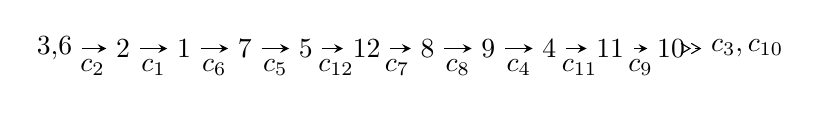
\begin{tikzpicture}[x=22pt, y=7pt]
	% node
	\node (A0) at (-1/8, 0) {3,6};
	\node (A1) at (1, 0) {2};
	\node (A2) at (2, 0) {1};
	\node (A3) at (3, 0) {7};
	\node (A4) at (4, 0) {5};
	\node (A5) at (5, 0) {12};
	\node (A6) at (6, 0) {8};
	\node (A7) at (7, 0) {9};
	\node (A8) at (8, 0) {4};
	\node (A9) at (9, 0) {11};
	\node (A10) at (10, 0) {10};
	\node (C1) at (1/2, -1) {$c_{2}$};
	\node (C2) at (3/2, -1) {$c_{1}$};
	\node (C3) at (5/2, -1) {$c_{6}$};
	\node (C4) at (7/2, -1) {$c_{5}$};
	\node (C5) at (9/2, -1) {$c_{12}$};
	\node (C6) at (11/2, -1) {$c_{7}$};
	\node (C7) at (13/2, -1) {$c_{8}$};
	\node (C8) at (15/2, -1) {$c_{4}$};
	\node (C9) at (17/2, -1) {$c_{11}$};
	\node (C10) at (19/2, -1) {$c_{9}$};
	\node (A11) at (45/4, 0) {$c_{3},c_{10}$};

	% edge
	\draw[->,>=stealth]	
	(A0) edge (A1) (A1) edge (A2) (A2) edge (A3) (A3) edge (A4) (A4) edge (A5) (A5) edge (A6) (A6) edge (A7) (A7) edge (A8) (A8) edge (A9) (A9) edge (A10) ;
	\draw[->>,>={angle 60}]	
	(A10) edge (A11);
\end{tikzpicture} \\ 

\end{tabular} \\

\footnotetext{
The image of knot diagram is generated by the software ``\textbf{Draw programme}" developed by Andrew Bartholomew(\url{http://www.layer8.co.uk/maths/draw/index.htm\#Running-draw}), where we modified some parts for our purpose(\url{https://github.com/CATsTAILs/LinksPainter}).
}\phantom \\ \newline 
\centering \textbf{Ideals for irreducible components\footnotemark of $X_{\text{par}}$} 
 
\begin{align*}
I^u_{1}&=\langle 
u^{60}- u^{59}+\cdots- u^2+1\rangle \\
\\
\end{align*}
\raggedright * 1 irreducible components of $\dim_{\mathbb{C}}=0$, with total 60 representations.\\
\footnotetext{All coefficients of polynomials are rational numbers. But the coefficients are sometimes approximated in decimal forms when there is not enough margin.}
\newpage
\renewcommand{\arraystretch}{1}
\centering \section*{I. $I^u_{1}= \langle u^{60}- u^{59}+\cdots- u^2+1 \rangle$}
\flushleft \textbf{(i) Arc colorings}\\
\begin{tabular}{m{7pt} m{180pt} m{7pt} m{180pt} }
\flushright $a_{3}=$&$\begin{pmatrix}1\\0\end{pmatrix}$ \\
\flushright $a_{6}=$&$\begin{pmatrix}0\\u\end{pmatrix}$ \\
\flushright $a_{2}=$&$\begin{pmatrix}1\\- u^2\end{pmatrix}$ \\
\flushright $a_{1}=$&$\begin{pmatrix}- u^2+1\\- u^2\end{pmatrix}$ \\
\flushright $a_{7}=$&$\begin{pmatrix}u^5-2 u^3+u\\u^5- u^3+u\end{pmatrix}$ \\
\flushright $a_{5}=$&$\begin{pmatrix}u\\- u^3+u\end{pmatrix}$ \\
\flushright $a_{12}=$&$\begin{pmatrix}- u^8+3 u^6-3 u^4+1\\- u^8+2 u^6-2 u^4\end{pmatrix}$ \\
\flushright $a_{8}=$&$\begin{pmatrix}u^{11}-4 u^9+6 u^7-2 u^5-3 u^3+2 u\\u^{11}-3 u^9+4 u^7- u^5- u^3+u\end{pmatrix}$ \\
\flushright $a_{9}=$&$\begin{pmatrix}- u^{15}+4 u^{13}-6 u^{11}+8 u^7-6 u^5-2 u^3+2 u\\u^{17}-5 u^{15}+11 u^{13}-10 u^{11}- u^9+10 u^7-6 u^5+u\end{pmatrix}$ \\
\flushright $a_{4}=$&$\begin{pmatrix}u^{29}-8 u^{27}+\cdots+2 u^3+u\\- u^{31}+9 u^{29}+\cdots-4 u^5+u\end{pmatrix}$ \\
\flushright $a_{11}=$&$\begin{pmatrix}- u^{14}+5 u^{12}-10 u^{10}+7 u^8+4 u^6-8 u^4+2 u^2+1\\- u^{14}+4 u^{12}-7 u^{10}+4 u^8+2 u^6-4 u^4+u^2\end{pmatrix}$ \\
\flushright $a_{10}=$&$\begin{pmatrix}u^{45}-14 u^{43}+\cdots-18 u^5+3 u\\u^{45}-13 u^{43}+\cdots+u^3+u\end{pmatrix}$\\&\end{tabular}
\flushleft \textbf{(ii) Obstruction class $= -1$}\\~\\
\flushleft \textbf{(iii) Cusp Shapes $= 4 u^{59}-72 u^{57}+\cdots-8 u-2$}\\~\\
\newpage\renewcommand{\arraystretch}{1}
\flushleft \textbf{(iv) u-Polynomials at the component}\newline \\
\begin{tabular}{m{50pt}|m{274pt}}
Crossings & \hspace{64pt}u-Polynomials at each crossing \\
\hline $$\begin{aligned}c_{1}\end{aligned}$$&$\begin{aligned}
&u^{60}+35 u^{59}+\cdots+2 u+1
\end{aligned}$\\
\hline $$\begin{aligned}c_{2},c_{5}\end{aligned}$$&$\begin{aligned}
&u^{60}+u^{59}+\cdots- u^2+1
\end{aligned}$\\
\hline $$\begin{aligned}c_{3},c_{10}\end{aligned}$$&$\begin{aligned}
&u^{60}+u^{59}+\cdots+2 u+1
\end{aligned}$\\
\hline $$\begin{aligned}c_{4},c_{8}\end{aligned}$$&$\begin{aligned}
&u^{60}+3 u^{59}+\cdots-453 u^2+77
\end{aligned}$\\
\hline $$\begin{aligned}c_{6},c_{7},c_{11}\\c_{12}\end{aligned}$$&$\begin{aligned}
&u^{60}+3 u^{59}+\cdots+34 u+5
\end{aligned}$\\
\hline $$\begin{aligned}c_{9}\end{aligned}$$&$\begin{aligned}
&u^{60}-31 u^{59}+\cdots-2 u+1
\end{aligned}$\\
\hline
\end{tabular}\\~\\
\newpage\renewcommand{\arraystretch}{1}
\flushleft \textbf{(v) Riley Polynomials at the component}\newline \\
\begin{tabular}{m{50pt}|m{274pt}}
Crossings & \hspace{64pt}Riley Polynomials at each crossing \\
\hline $$\begin{aligned}c_{1}\end{aligned}$$&$\begin{aligned}
&y^{60}-19 y^{59}+\cdots-10 y+1
\end{aligned}$\\
\hline $$\begin{aligned}c_{2},c_{5}\end{aligned}$$&$\begin{aligned}
&y^{60}-35 y^{59}+\cdots-2 y+1
\end{aligned}$\\
\hline $$\begin{aligned}c_{3},c_{10}\end{aligned}$$&$\begin{aligned}
&y^{60}-31 y^{59}+\cdots-2 y+1
\end{aligned}$\\
\hline $$\begin{aligned}c_{4},c_{8}\end{aligned}$$&$\begin{aligned}
&y^{60}+37 y^{59}+\cdots-69762 y+5929
\end{aligned}$\\
\hline $$\begin{aligned}c_{6},c_{7},c_{11}\\c_{12}\end{aligned}$$&$\begin{aligned}
&y^{60}+73 y^{59}+\cdots+74 y+25
\end{aligned}$\\
\hline $$\begin{aligned}c_{9}\end{aligned}$$&$\begin{aligned}
&y^{60}-3 y^{59}+\cdots-2 y+1
\end{aligned}$\\
\hline
\end{tabular}\\~\\
\newpage\flushleft \textbf{(vi) Complex Volumes and Cusp Shapes}
$$\begin{array}{c|c|c}  
\text{Solutions to }I^u_{1}& \I (\text{vol} + \sqrt{-1}CS) & \text{Cusp shape}\\
 \hline 
\begin{aligned}
u &= -0.919475 + 0.342245 I\end{aligned}
 & \phantom{-}0.08563 + 3.24816 I & \phantom{-}2.86695 - 8.06640 I \\ \hline\begin{aligned}
u &= -0.919475 - 0.342245 I\end{aligned}
 & \phantom{-}0.08563 - 3.24816 I & \phantom{-}2.86695 + 8.06640 I \\ \hline\begin{aligned}
u &= -1.044190 + 0.193501 I\end{aligned}
 & \phantom{-}0.32484 + 3.60424 I & -1.15833 - 4.66740 I \\ \hline\begin{aligned}
u &= -1.044190 - 0.193501 I\end{aligned}
 & \phantom{-}0.32484 - 3.60424 I & -1.15833 + 4.66740 I \\ \hline\begin{aligned}
u &= \phantom{-}0.905641 + 0.075866 I\end{aligned}
 & -1.51462 - 0.22405 I & -6.40245 + 0.27111 I \\ \hline\begin{aligned}
u &= \phantom{-}0.905641 - 0.075866 I\end{aligned}
 & -1.51462 + 0.22405 I & -6.40245 - 0.27111 I \\ \hline\begin{aligned}
u &= -0.006041 + 0.904852 I\end{aligned}
 & -10.02580 - 2.42359 I & -2.65635 + 3.19391 I \\ \hline\begin{aligned}
u &= -0.006041 - 0.904852 I\end{aligned}
 & -10.02580 + 2.42359 I & -2.65635 - 3.19391 I \\ \hline\begin{aligned}
u &= \phantom{-}0.038465 + 0.899651 I\end{aligned}
 & -4.64353 + 8.98999 I & \phantom{-}1.72039 - 5.67712 I \\ \hline\begin{aligned}
u &= \phantom{-}0.038465 - 0.899651 I\end{aligned}
 & -4.64353 - 8.98999 I & \phantom{-}1.72039 + 5.67712 I \\ \hline\begin{aligned}
u &= -0.030149 + 0.897007 I\end{aligned}
 & -7.37251 - 4.03814 I & -1.44998 + 2.20533 I \\ \hline\begin{aligned}
u &= -0.030149 - 0.897007 I\end{aligned}
 & -7.37251 + 4.03814 I & -1.44998 - 2.20533 I \\ \hline\begin{aligned}
u &= \phantom{-}0.763924 + 0.465497 I\end{aligned}
 & \phantom{-}5.00437 - 6.11953 I & \phantom{-}7.26352 + 7.85803 I \\ \hline\begin{aligned}
u &= \phantom{-}0.763924 - 0.465497 I\end{aligned}
 & \phantom{-}5.00437 + 6.11953 I & \phantom{-}7.26352 - 7.85803 I \\ \hline\begin{aligned}
u &= \phantom{-}0.030712 + 0.880798 I\end{aligned}
 & -3.02518 + 0.62968 I & \phantom{-}3.76609 + 0.36863 I \\ \hline\begin{aligned}
u &= \phantom{-}0.030712 - 0.880798 I\end{aligned}
 & -3.02518 - 0.62968 I & \phantom{-}3.76609 - 0.36863 I \\ \hline\begin{aligned}
u &= \phantom{-}1.092890 + 0.282962 I\end{aligned}
 & -3.07831 - 0.54807 I & \phantom{-0.000000 } 0 \\ \hline\begin{aligned}
u &= \phantom{-}1.092890 - 0.282962 I\end{aligned}
 & -3.07831 + 0.54807 I & \phantom{-0.000000 } 0 \\ \hline\begin{aligned}
u &= \phantom{-}1.032740 + 0.462956 I\end{aligned}
 & \phantom{-}2.05457 - 2.50514 I & \phantom{-0.000000 } 0 \\ \hline\begin{aligned}
u &= \phantom{-}1.032740 - 0.462956 I\end{aligned}
 & \phantom{-}2.05457 + 2.50514 I & \phantom{-0.000000 } 0 \\ \hline\begin{aligned}
u &= -0.739994 + 0.426951 I\end{aligned}
 & \phantom{-}1.82247 + 1.86091 I & \phantom{-}4.36406 - 4.47008 I \\ \hline\begin{aligned}
u &= -0.739994 - 0.426951 I\end{aligned}
 & \phantom{-}1.82247 - 1.86091 I & \phantom{-}4.36406 + 4.47008 I \\ \hline\begin{aligned}
u &= -1.117990 + 0.254452 I\end{aligned}
 & -0.50349 - 3.93794 I & \phantom{-0.000000 } 0 \\ \hline\begin{aligned}
u &= -1.117990 - 0.254452 I\end{aligned}
 & -0.50349 + 3.93794 I & \phantom{-0.000000 } 0 \\ \hline\begin{aligned}
u &= -1.062020 + 0.457339 I\end{aligned}
 & -1.79262 + 6.16892 I & \phantom{-0.000000 } 0 \\ \hline\begin{aligned}
u &= -1.062020 - 0.457339 I\end{aligned}
 & -1.79262 - 6.16892 I & \phantom{-0.000000 } 0 \\ \hline\begin{aligned}
u &= \phantom{-}0.701269 + 0.462491 I\end{aligned}
 & \phantom{-}5.17636 + 2.18925 I & \phantom{-}8.10847 + 0.13060 I \\ \hline\begin{aligned}
u &= \phantom{-}0.701269 - 0.462491 I\end{aligned}
 & \phantom{-}5.17636 - 2.18925 I & \phantom{-}8.10847 - 0.13060 I \\ \hline\begin{aligned}
u &= \phantom{-}1.109480 + 0.360438 I\end{aligned}
 & -4.69760 - 1.44356 I & \phantom{-0.000000 } 0 \\ \hline\begin{aligned}
u &= \phantom{-}1.109480 - 0.360438 I\end{aligned}
 & -4.69760 + 1.44356 I & \phantom{-0.000000 } 0\\
 \hline 
 \end{array}$$\newpage$$\begin{array}{c|c|c}  
\text{Solutions to }I^u_{1}& \I (\text{vol} + \sqrt{-1}CS) & \text{Cusp shape}\\
 \hline 
\begin{aligned}
u &= \phantom{-}1.065550 + 0.475941 I\end{aligned}
 & \phantom{-}1.11940 - 10.83400 I & \phantom{-0.000000 } 0 \\ \hline\begin{aligned}
u &= \phantom{-}1.065550 - 0.475941 I\end{aligned}
 & \phantom{-}1.11940 + 10.83400 I & \phantom{-0.000000 } 0 \\ \hline\begin{aligned}
u &= -1.104060 + 0.403777 I\end{aligned}
 & -4.38057 + 5.70362 I & \phantom{-0.000000 } 0 \\ \hline\begin{aligned}
u &= -1.104060 - 0.403777 I\end{aligned}
 & -4.38057 - 5.70362 I & \phantom{-0.000000 } 0 \\ \hline\begin{aligned}
u &= \phantom{-}0.255046 + 0.618563 I\end{aligned}
 & \phantom{-}3.38358 + 6.59803 I & \phantom{-}5.15553 - 6.30688 I \\ \hline\begin{aligned}
u &= \phantom{-}0.255046 - 0.618563 I\end{aligned}
 & \phantom{-}3.38358 - 6.59803 I & \phantom{-}5.15553 + 6.30688 I \\ \hline\begin{aligned}
u &= -1.257920 + 0.450457 I\end{aligned}
 & -6.94466 + 4.07293 I & \phantom{-0.000000 } 0 \\ \hline\begin{aligned}
u &= -1.257920 - 0.450457 I\end{aligned}
 & -6.94466 - 4.07293 I & \phantom{-0.000000 } 0 \\ \hline\begin{aligned}
u &= \phantom{-}1.249740 + 0.482651 I\end{aligned}
 & -6.70940 - 5.51033 I & \phantom{-0.000000 } 0 \\ \hline\begin{aligned}
u &= \phantom{-}1.249740 - 0.482651 I\end{aligned}
 & -6.70940 + 5.51033 I & \phantom{-0.000000 } 0 \\ \hline\begin{aligned}
u &= \phantom{-}1.267950 + 0.452530 I\end{aligned}
 & -11.34370 - 0.73251 I & \phantom{-0.000000 } 0 \\ \hline\begin{aligned}
u &= \phantom{-}1.267950 - 0.452530 I\end{aligned}
 & -11.34370 + 0.73251 I & \phantom{-0.000000 } 0 \\ \hline\begin{aligned}
u &= -1.270740 + 0.447700 I\end{aligned}
 & -8.65827 - 4.23519 I & \phantom{-0.000000 } 0 \\ \hline\begin{aligned}
u &= -1.270740 - 0.447700 I\end{aligned}
 & -8.65827 + 4.23519 I & \phantom{-0.000000 } 0 \\ \hline\begin{aligned}
u &= -1.257410 + 0.485584 I\end{aligned}
 & -11.0988 + 8.9801 I & \phantom{-0.000000 } 0 \\ \hline\begin{aligned}
u &= -1.257410 - 0.485584 I\end{aligned}
 & -11.0988 - 8.9801 I & \phantom{-0.000000 } 0 \\ \hline\begin{aligned}
u &= \phantom{-}1.256940 + 0.490183 I\end{aligned}
 & -8.3433 - 13.9630 I & \phantom{-0.000000 } 0 \\ \hline\begin{aligned}
u &= \phantom{-}1.256940 - 0.490183 I\end{aligned}
 & -8.3433 + 13.9630 I & \phantom{-0.000000 } 0 \\ \hline\begin{aligned}
u &= \phantom{-}1.268500 + 0.467782 I\end{aligned}
 & -13.92050 - 2.45161 I & \phantom{-0.000000 } 0 \\ \hline\begin{aligned}
u &= \phantom{-}1.268500 - 0.467782 I\end{aligned}
 & -13.92050 + 2.45161 I & \phantom{-0.000000 } 0 \\ \hline\begin{aligned}
u &= -1.266320 + 0.474454 I\end{aligned}
 & -13.8709 + 7.3329 I & \phantom{-0.000000 } 0 \\ \hline\begin{aligned}
u &= -1.266320 - 0.474454 I\end{aligned}
 & -13.8709 - 7.3329 I & \phantom{-0.000000 } 0 \\ \hline\begin{aligned}
u &= \phantom{-}0.306849 + 0.559155 I\end{aligned}
 & \phantom{-}4.05629 - 1.56504 I & \phantom{-}7.07085 + 0.73954 I \\ \hline\begin{aligned}
u &= \phantom{-}0.306849 - 0.559155 I\end{aligned}
 & \phantom{-}4.05629 + 1.56504 I & \phantom{-}7.07085 - 0.73954 I \\ \hline\begin{aligned}
u &= -0.234349 + 0.574464 I\end{aligned}
 & \phantom{-}0.48435 - 2.11140 I & \phantom{-}1.91014 + 3.36891 I \\ \hline\begin{aligned}
u &= -0.234349 - 0.574464 I\end{aligned}
 & \phantom{-}0.48435 + 2.11140 I & \phantom{-}1.91014 - 3.36891 I \\ \hline\begin{aligned}
u &= -0.061807 + 0.591217 I\end{aligned}
 & -1.52087 - 1.95278 I & -1.21392 + 4.59969 I \\ \hline\begin{aligned}
u &= -0.061807 - 0.591217 I\end{aligned}
 & -1.52087 + 1.95278 I & -1.21392 - 4.59969 I \\ \hline\begin{aligned}
u &= -0.473230 + 0.288232 I\end{aligned}
 & \phantom{-}1.236790 - 0.098801 I & \phantom{-}8.77548 + 0.26744 I \\ \hline\begin{aligned}
u &= -0.473230 - 0.288232 I\end{aligned}
 & \phantom{-}1.236790 + 0.098801 I & \phantom{-}8.77548 - 0.26744 I\\
 \hline 
 \end{array}$$\newpage
\newpage\renewcommand{\arraystretch}{1}
\centering \section*{ II. u-Polynomials}
\begin{tabular}{m{50pt}|m{274pt}}
Crossings & \hspace{64pt}u-Polynomials at each crossing \\
\hline $$\begin{aligned}c_{1}\end{aligned}$$&$\begin{aligned}
&u^{60}+35 u^{59}+\cdots+2 u+1
\end{aligned}$\\
\hline $$\begin{aligned}c_{2},c_{5}\end{aligned}$$&$\begin{aligned}
&u^{60}+u^{59}+\cdots- u^2+1
\end{aligned}$\\
\hline $$\begin{aligned}c_{3},c_{10}\end{aligned}$$&$\begin{aligned}
&u^{60}+u^{59}+\cdots+2 u+1
\end{aligned}$\\
\hline $$\begin{aligned}c_{4},c_{8}\end{aligned}$$&$\begin{aligned}
&u^{60}+3 u^{59}+\cdots-453 u^2+77
\end{aligned}$\\
\hline $$\begin{aligned}c_{6},c_{7},c_{11}\\c_{12}\end{aligned}$$&$\begin{aligned}
&u^{60}+3 u^{59}+\cdots+34 u+5
\end{aligned}$\\
\hline $$\begin{aligned}c_{9}\end{aligned}$$&$\begin{aligned}
&u^{60}-31 u^{59}+\cdots-2 u+1
\end{aligned}$\\
\hline
\end{tabular}\newpage\renewcommand{\arraystretch}{1}
\centering \section*{ III. Riley Polynomials}
\begin{tabular}{m{50pt}|m{274pt}}
Crossings & \hspace{64pt}Riley Polynomials at each crossing \\
\hline $$\begin{aligned}c_{1}\end{aligned}$$&$\begin{aligned}
&y^{60}-19 y^{59}+\cdots-10 y+1
\end{aligned}$\\
\hline $$\begin{aligned}c_{2},c_{5}\end{aligned}$$&$\begin{aligned}
&y^{60}-35 y^{59}+\cdots-2 y+1
\end{aligned}$\\
\hline $$\begin{aligned}c_{3},c_{10}\end{aligned}$$&$\begin{aligned}
&y^{60}-31 y^{59}+\cdots-2 y+1
\end{aligned}$\\
\hline $$\begin{aligned}c_{4},c_{8}\end{aligned}$$&$\begin{aligned}
&y^{60}+37 y^{59}+\cdots-69762 y+5929
\end{aligned}$\\
\hline $$\begin{aligned}c_{6},c_{7},c_{11}\\c_{12}\end{aligned}$$&$\begin{aligned}
&y^{60}+73 y^{59}+\cdots+74 y+25
\end{aligned}$\\
\hline $$\begin{aligned}c_{9}\end{aligned}$$&$\begin{aligned}
&y^{60}-3 y^{59}+\cdots-2 y+1
\end{aligned}$\\
\hline
\end{tabular}
\vskip 2pc
\end{document}